% !TEX root=../main.tex
\begin{lecture}[Lévy sampling]
    Опять же, мы все работаем с стат.суммами $Z(\beta)$.

    \section{Наивное сэмплирование}
    На прошлой неделе алгоритмы сэмплирования \textit{пути} имели ненулевой rejection rate.
    Иными словами, часть предложенных движений отвергалась (например, в листинге \ref{code:naive_harmonic_path}).

    \pythonfile{../w6/programs_lecture_6/naive_path_slice}{Программа для сэмплирования вдоль одного фиксированного среза $x_k$ (\texttt{naive\_path\_slice.py})}{code:naive_path_slice}

    Существует алгоритм \textit{без отвержения} конфигураций (Lévy sampling).
    Его идею проще понять на примере свободной частицы.

    \section{Lévy sampling для свободной частицы}
    \subsection{Гауссианы}

    Для свободной частицы проводится сэмплирование по алгоритму Метрополиса (как в \ref{code:naive_path_slice}).
    Получающиеся координаты имеют распределение по Гауссу, так как $\rho^{\text{free}} (x, x', \beta)$ имеет форму гауссианы (см. \eqref{eq:rho-free-particle}).
    Более формально, для вероятности имеем $\pi (x_k | x_{k-1}, x_{k+1}) \propto \rho^{\text{free}} (x_{k-1}, x_k, \Delta \tau) \rho^{\text{free}} (x_k, x_{k+1}, \Delta \tau)$, что есть гауссиана, причем:
    \begin{align}
        \label{eq:pi-x_k-when-k-fixed}
        & \pi (x_k) = \exp\left(- \frac{(x_k - \braket{x_k})^2}{2\sigma^2}\right),
        & \braket{x_k} = \frac{x_{k+1} + x_{k-1}}{2}, \, 
        & \sigma^2 = \frac{\Delta \tau}{2} 
    \end{align}

    А поскольку распределие идет по гауссиане, имеет смысл сэмплировать $x_k$ из гауссианы.
    Но это еще не все.
    Мы знаем, что вероятность подчиняется формуле:
    \begin{equation}
        \label{eq:pi_free-x'-x''}
        \pi^{\mathrm{free}}\left(x_{k} \mid x^{\prime}, x^{\prime \prime}\right) \propto \rho^{\mathrm{free}}\left(x^{\prime}, x_{k}, \Delta_{\tau}^{\prime}\right) \rho^{\mathrm{free}}\left(x_{k}, x^{\prime \prime}, \Delta_{\tau}^{\prime \prime}\right)
    \end{equation}
    Это произведение гауссиан --- то есть, тоже гауссиана с характеристиками:
    \begin{align}
        \label{eq:gauss-params-slice-x'-x''-mean}
        \left\langle x_{k}\right\rangle &=
        \frac{\Delta_{\tau}^{\prime \prime} x^{\prime}+\Delta_{\tau}^{\prime} x^{\prime \prime}}{\Delta_{\tau}^{\prime \prime}+\Delta_{\tau}^{\prime}} \\ \sigma^{2} &=
        \label{eq:gauss-params-slice-x'-x''-sigma}
        \left(\frac{1}{\Delta_{\tau}^{\prime \prime}}+\frac{1}{\Delta_{\tau}^{\prime}}\right)^{-1}
    \end{align}
    
    Построим теперь путь из $x_0$ в $x_N$ следующим образом.
    \subsection{Алгоритм}
    \label{enum:levy-algorithm}
    \begin{enumerate}
        \item Выберем $x_1$ по гауссиане с заданными соседями ($x_0$, $x_N$), т.е. как $\pi (x | x_0, x_N)$ (рис. \ref{fig:x_1-levy_example}), причем для $x_N$ берем $\beta = \frac{N-1}{N}\,$.
        \item Повторим процедуру для $x_2$, выбирая его между $(x_1, x_N)$.
            На этот раз для $x_N$ берем $\beta = \frac{N-2}{N}\,$.
        \item Повторяем, пока не получим весь путь.
    \end{enumerate}

    \begin{figure}[ht]
        \begin{subfigure}{0.33\columnwidth}
            \centering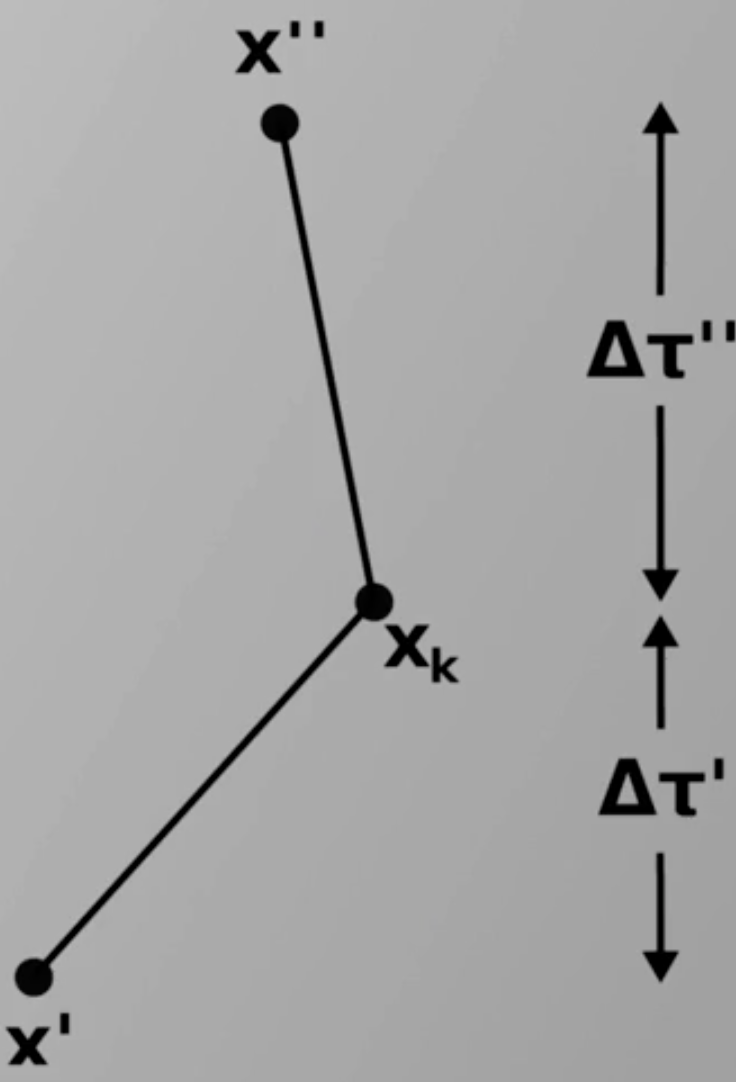
\includegraphics[width=\linewidth]{fig/path-slice}
            \caption{Путь $x' \rightarrow x_k \rightarrow x''$}
            \label{fig:x_k-between-primes}
        \end{subfigure}
        \begin{subfigure}{0.33\columnwidth}
            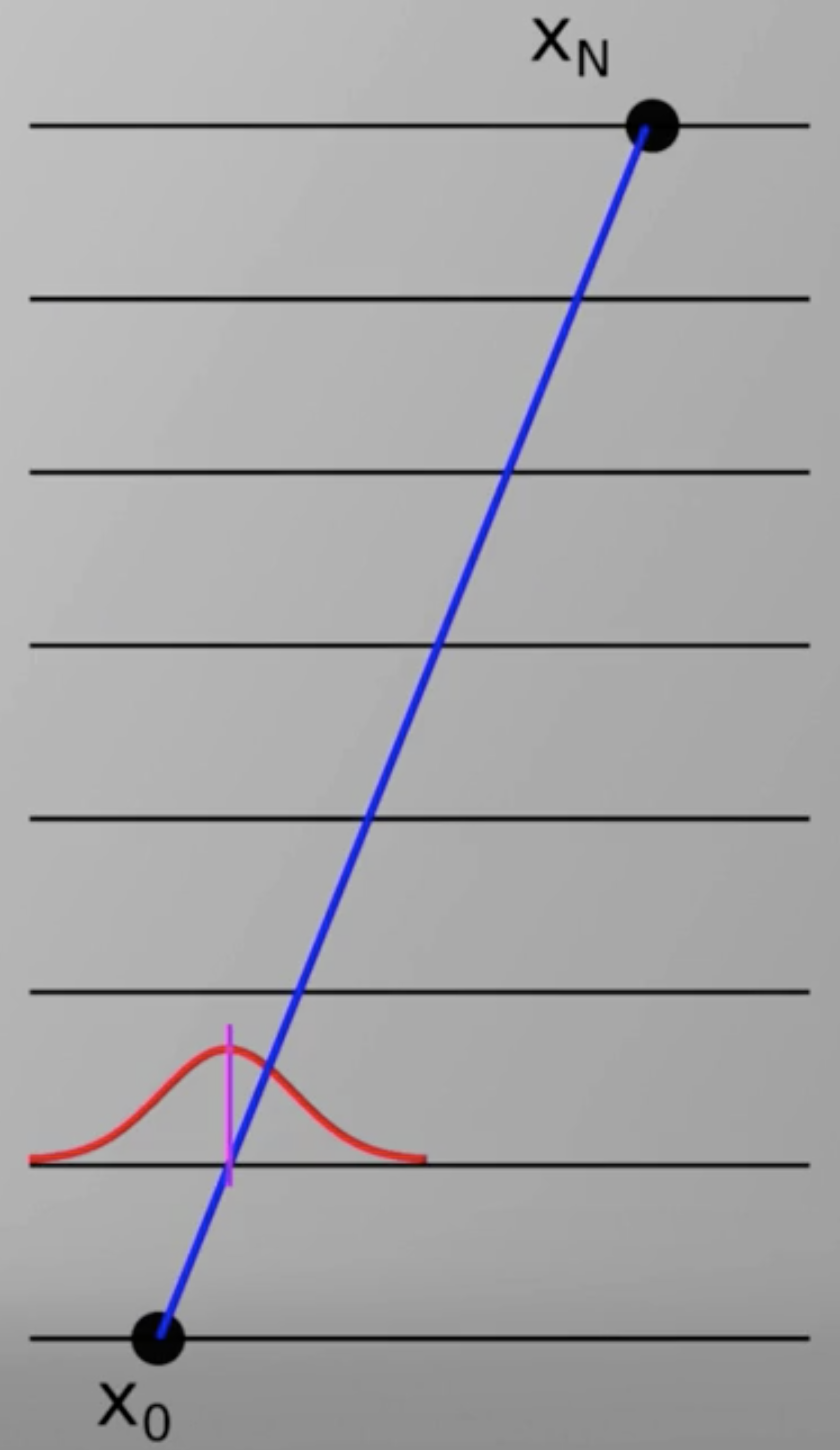
\includegraphics[width=\linewidth]{fig/x1-selection}
            \caption{Сэмплирование $x_1$ через точки $x_0, x_N$}
            \label{fig:x_1-levy_example}
        \end{subfigure}
        \begin{subfigure}{0.33\columnwidth}
            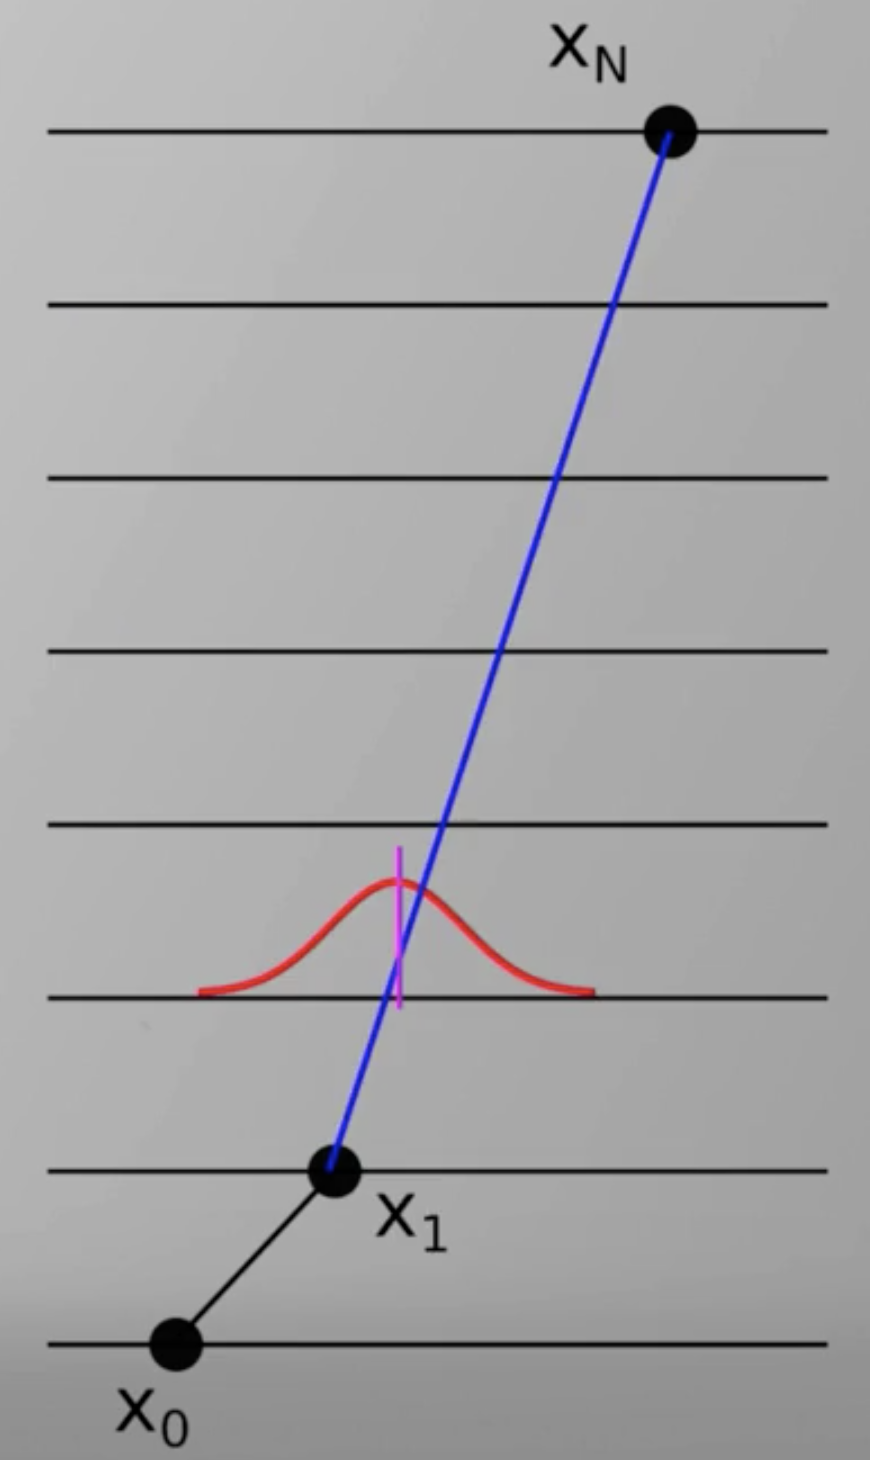
\includegraphics[width=\linewidth]{fig/x2-selection}
            \caption{Сэмплирование $x_2$ через точки $x_1, x_N$}
            \label{fig:x_2-levy_example}
        \end{subfigure}
        \caption{Пример Lévy sampling}
        \label{fig:x_k-levy-sampling}
    \end{figure}

    Утверждается, что полученный алгоритм приводит к такому же распределению, как и в коде \ref{code:naive_path_slice}.
    Попробуем это понять.

    \subsection{Обсуждение алгоритма}

    По свойству конволюции \eqref{eq:rho_convolution-derivation} мы можем разбить путь на два подпути:
    \begin{equation}
        \label{eq:levy_proof-path_split-x_1}
        \rho (x_0, x_N, \beta) = \int dx_1 {\color{blue} \rho(x_0, x_1, \beta /N)} {\color{red} \rho\left(x_1, x_N, \beta \frac{N-1}{N}\,\right)}
    \end{equation}
    Этот интеграл сводим к сумме по путям, как делалось в прошлой лекции:
    \begin{equation}
        \label{eq:levy_proof-path_split-x_1-discrete}
        \rho(x_0, x_N, \beta) = \Delta V \sum\limits_{x_1 \in \text{grid}}^{} {\color{blue} \rho(x_0, x_1, \beta /N)} {\color{red} \rho\left(x_1, x_N, \beta \frac{N-1}{N}\,\right)}
    \end{equation}

    $x_1$ здесь будет сэмплироваться по алгоритму выше между точками $(x_1, x_N)$ и с $\beta'' = \frac{N-1}{N}\,\beta$ по выражению \eqref{eq:gauss-params-slice-x'-x''-mean}.
    По идее, здесь мы могли бы и ограничиться: у нас есть путь $x_0 \rightarrow x_1 \rightarrow x_N$ длиной в три точки и мы можем просто сэмплировать $x_1$ по гауссиане с параметрами из \eqref{eq:pi_free-x'-x''}-\eqref{eq:gauss-params-slice-x'-x''-sigma}.
    Но наша цель --- получить $\beta /N$ (для разложения Trotter в дальнейшем), поэтому поработаем со вторым множителем:
    \begin{equation}
        \label{eq:levy_proof-recursive_decomposition}
        {\color{red} \rho\left(x_1, x_N, \beta \frac{N-1}{N}\,\right)} =
        \Delta V \sum\limits_{x_2 \in \text{grid}}^{} \rho(x_1, x_2, \beta /N) \rho\left( x_2, x_N, \beta \frac{N-2}{N}\, \right) 
    \end{equation}

    Этим действием мы ввели еще одну переменную $x_2$ и \textbf{уменьшили множитель $\frac{N-1}{N}\,\beta$ до $\frac{N-2}{N}\,\beta$}.
    Переменная $x_2$ будет сэмлироваться точно так же по гауссиане, но уже между точками $(x_1, x_N)$ и с поправленной $\beta'' = \frac{N-2}{N}\, \beta$.

    Ясно, что этот процесс мы можем повторять до тех пор, пока не дойдем до $x_{N-1}$ и $\beta''$ не уменьшится до $\beta'' = \beta /N$.
    Этим мы добьемся поставленной цели уменьшить $\beta$ --- и на этом как раз завершается приведенный выше алгоритм.

    Реализация на Питоне можно увидеть в листинге \ref{code:levy_free_path}.

    \pythonfile{../w6/programs_lecture_6/levy_free_path}{Lévy sampling для свободной частицы (\texttt{levy\_free\_path.py})}{code:levy_free_path}

    \subsection{Random walk and Lévy sampling}
    Существует упрощение алгоритма.
    Не будем требовать, чтобы конечная точка $x''$ в точности совпадала с $x_N$, а на каждом этапе будем брать $\braket{x_k} = x_{k-1}$ вместо выражения \eqref{eq:gauss-params-slice-x'-x''-mean}.
    С одной стороны, мы получим случайные блуждания (см. рис. \ref{fig:random-walk} и код \ref{code:continuous_random_walk}).
    \pythonfile{../w6/programs_lecture_6/continuous_random_walk}{Случайные блуждания (\texttt{continuous\_random\_walk.py})}{code:continuous_random_walk}
    С другой стороны, полученную картину можно <<стянуть>> к точке $x_N$, сдвинув верхнюю точку (в случае \ref{fig:random-walk-pulling} двигать надо влево) на $| x_N - x' |$, а промежуточные точки --- на величину, пропорциональную $\frac{\tau}{\beta}\,|x_N - x'|$.
    Можно показать, что этот алгоритм даст такое же распределние, как и оригинальный Леви (\textit{я не смог доказать}).
    Код полученного упрощения приведен на \ref{code:trivial_free_path}.

    \pythonfile{../w6/programs_lecture_6/continuous_random_walk}{Lévy sampling через случайные блуждания (\texttt{continuous\_random\_walk.py})}{code:trivial_free_path}
    \begin{figure}[ht]
        \begin{subfigure}{0.5\columnwidth}
            \centering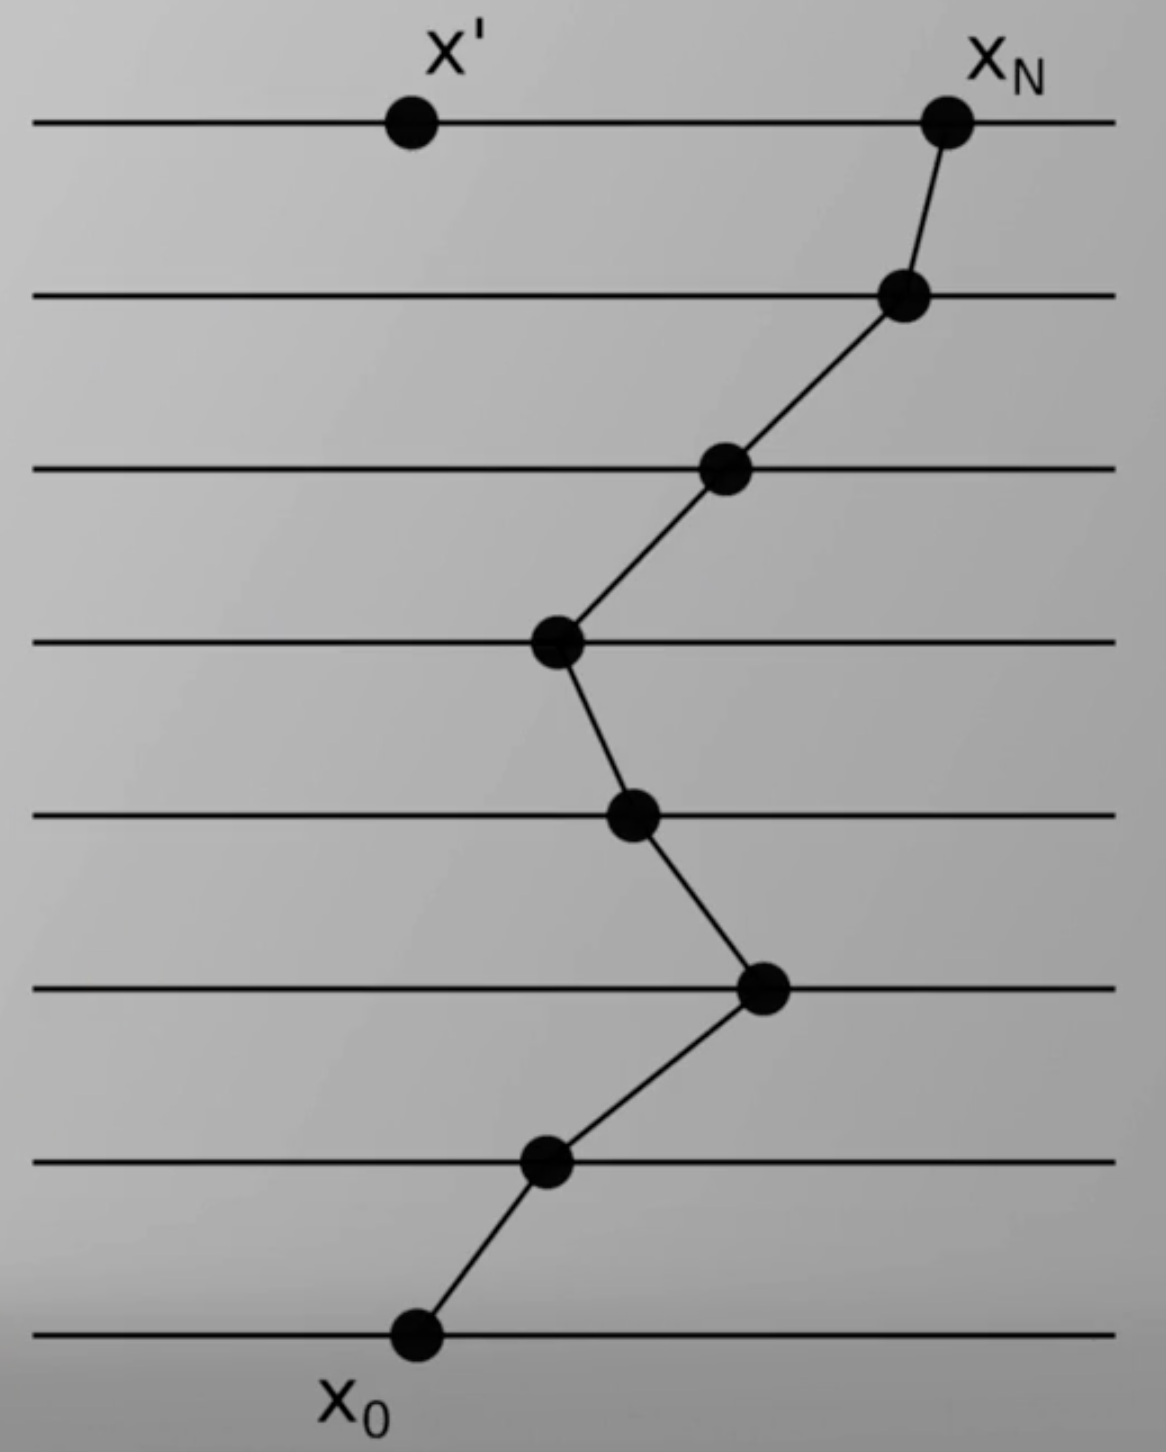
\includegraphics[width=\linewidth]{fig/random-walk}
            \caption{Случайное блуждание без фиксации $x_N$ в качестве конечной точки}
            \label{fig:random-walk}
        \end{subfigure}
        \begin{subfigure}{0.5\columnwidth}
            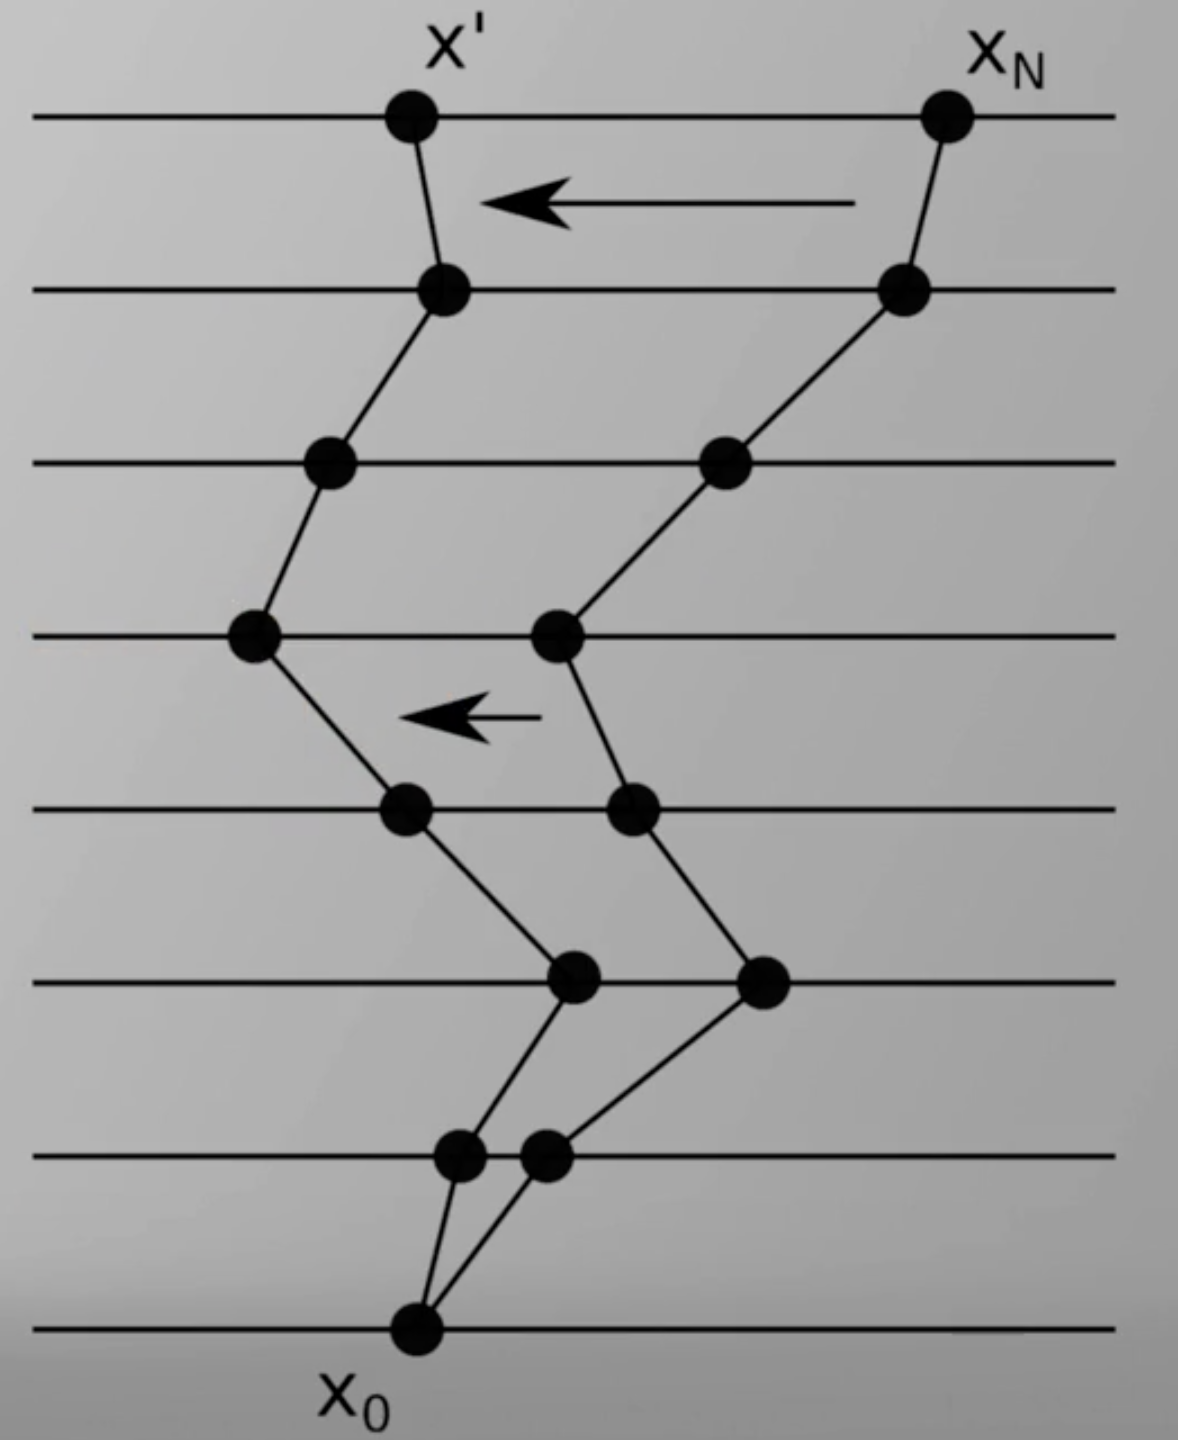
\includegraphics[width=\linewidth]{fig/random-walk-pulling}
            \caption{<<Стягивание>> случайного блуждания в точку $x_N$}
            \label{fig:random-walk-pulling}
        \end{subfigure}
        \caption{Сведение Random walk к Lévy sampling}
    \end{figure}

    \section{Lévy sampling для гармонического потенциала}
    \label{sec:levy-harmonic}
    Выведенный в предыдущем параграфе Lévy sampling сильно держится на том, что $\rho (x, x', \beta)$ свободной частицы есть гауссиана.
    Если же частица находится в потенциале $V(x)$, то рассуждения выше, вообще говоря, не работают.

    Однако в Trotter approximation для гармонического потенциала мы все еще имеем экспоненту как произведение трех экспонент:
    \begin{equation}
        \label{eq:rho_harmonic-trotter}
        \rho^{\text{harm}} (x, x', \beta) = e^{-\frac{\beta}{4}\, x^2} \rho^{\text{free}} (x, x', \beta) e^{-\frac{\beta}{4}\, {x'}^2}
    \end{equation}

    Это произведение трех экспонент можно переписать в подгоночном виде (теорфиз же!), для которого существует аналитическое решение:
    \begin{align}
        \label{eq:rho_harmonic-analytical}
        \rho^{\mathrm{harm}}\left(x, x^{\prime}, \beta\right) &= c(\beta) e^{-g(\beta) \frac{\left(x-x^{\prime}\right)^{2}}{2}} e^{-f(\beta) \frac{\left(x+x^{\prime}\right)^{2}}{2}} \\
        \label{eq:rho_harmonic-analytical-g}
        g(\beta) &= \frac{1}{2} \operatorname{coth} \frac{\beta}{2} \\ 
        \label{eq:rho_harmonic-analytical-f}
        f(\beta) &=\frac{1}{2} \tanh \frac{\beta}{2} \\ 
        \label{eq:rho_harmonic-analytical-c}
        c(\beta) &=\sqrt{\frac{1}{2 \pi \sinh \beta}} \\
        \label{eq:rho_harmonic-analytical-diagonal_element}
        \rho (x, x, \beta) &= \frac{1}{\sqrt{2\pi} \sqrt{\sinh \beta}}\,\exp\left( -x^2 \tanh(\beta /2) \right)
    \end{align}

    Напомним, что
    \begin{equation}
        \label{eq:gauss-distribution}
        f(x) = N(\mu, \sigma^2) = \frac{1}{\sigma \sqrt{2 \pi}} e^{-\frac{(x-\mu)^{2}}{2 \sigma^{2}}}
    \end{equation}

    Обратите внимание, что \eqref{eq:rho_harmonic-analytical-diagonal_element} не имеет вид гауссового распределения \eqref{eq:gauss-distribution}.
    Но можно показать (\textit{чуть-чуть посидеть и вывести}), что
    \begin{align}
        \label{eq:rho_harmonic-analytical-diagonal_element-via-gaussian}
        & \rho(x, x, \beta) = \frac{1}{\sqrt{2\tanh(\beta /2)} \sqrt{\sinh \beta}\,} N\left(0, \frac{1}{2\tanh (\beta /2)}\right),
        & \mu = 0,\,
        \sigma = \sqrt{\frac{1}{2\tanh(\beta /2)}}
    \end{align}

    Раз мы имеем дело с гауссианами, то можно применить всю Lévy-кухню к гармоническому потенциалу.
    Это реализовано в коде \ref{code:levy_harmonic_path}, где Ups1 есть $1 / \sigma^2$, а Ups2 есть хрен знает что.
    Я так и не смог понять, почему делится на $\sinh(\beta /N)$, а не $\tanh(\beta /N)$ и почему в дисперсии стоит $\tanh(\beta /N)$, а не $\tanh\left(\frac{\beta}{2}\,N\right)$.

    \pythonfile{../w6/programs_lecture_6/levy_harmonic_path}{Lévy sampling для гармонического осциллятора (\texttt{levy\_harmonic\_path.py})}{code:levy_harmonic_path}

    Не уверен, что гармонический Леви потом пригодится, поэтому мб не стоит над ним так запариваться.
\end{lecture}
